Neben den beiden selbst erzeugten Szenarien, werden nun Szenarien betrachtet, in denen die Terrain-Generierung der Blocklib genutzt wird. Für die Generierung nutzt die Blocklib einen Pseudo-Zufallszahlengenerator. Das ist ein Algorithmus, der ausgehend von einem übergebenen Wert, dem sogenannten \emph{Seed} Werte erzeugt, die zufällig \emph{wirken}. Der Algorithmus ist allerdings deterministisch. Mit dem selben Seed wird immer die selbe Folge von Zahlen generiert.

\begin{figure}
	\centering
	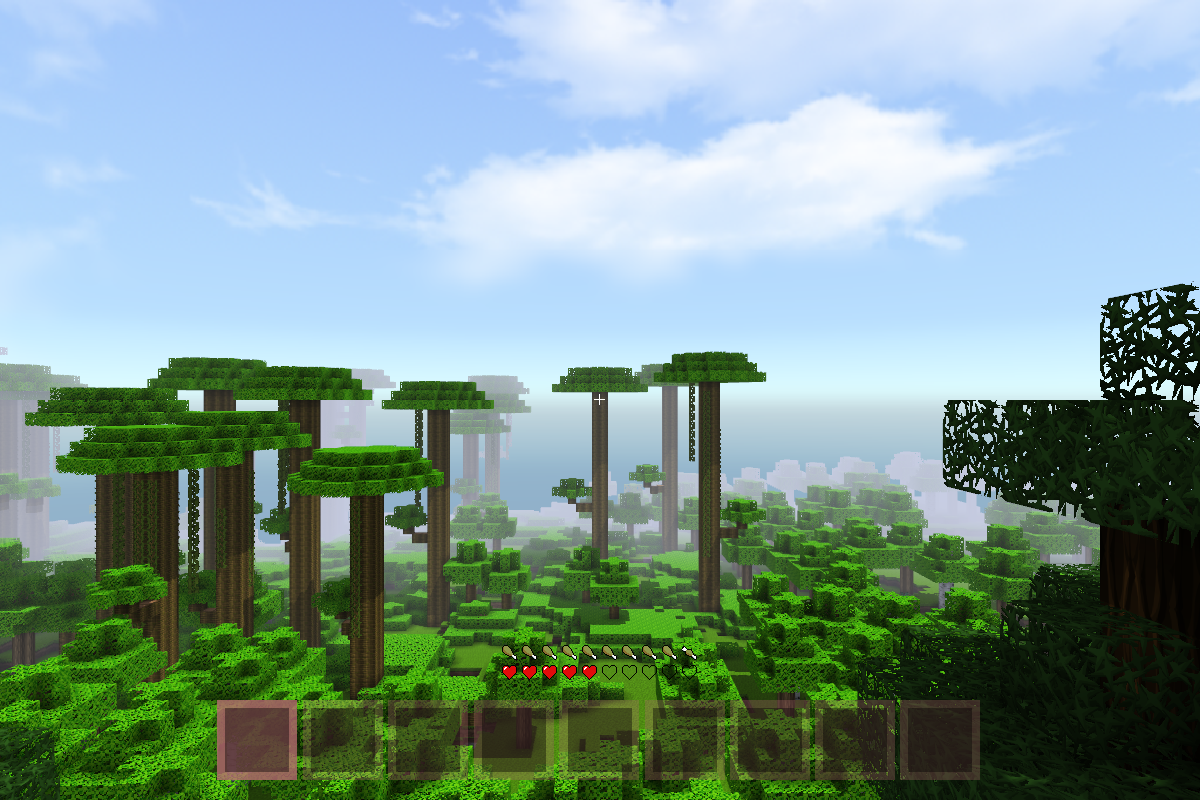
\includegraphics[width=.49\textwidth]{seed-0.png}
	\hfill
	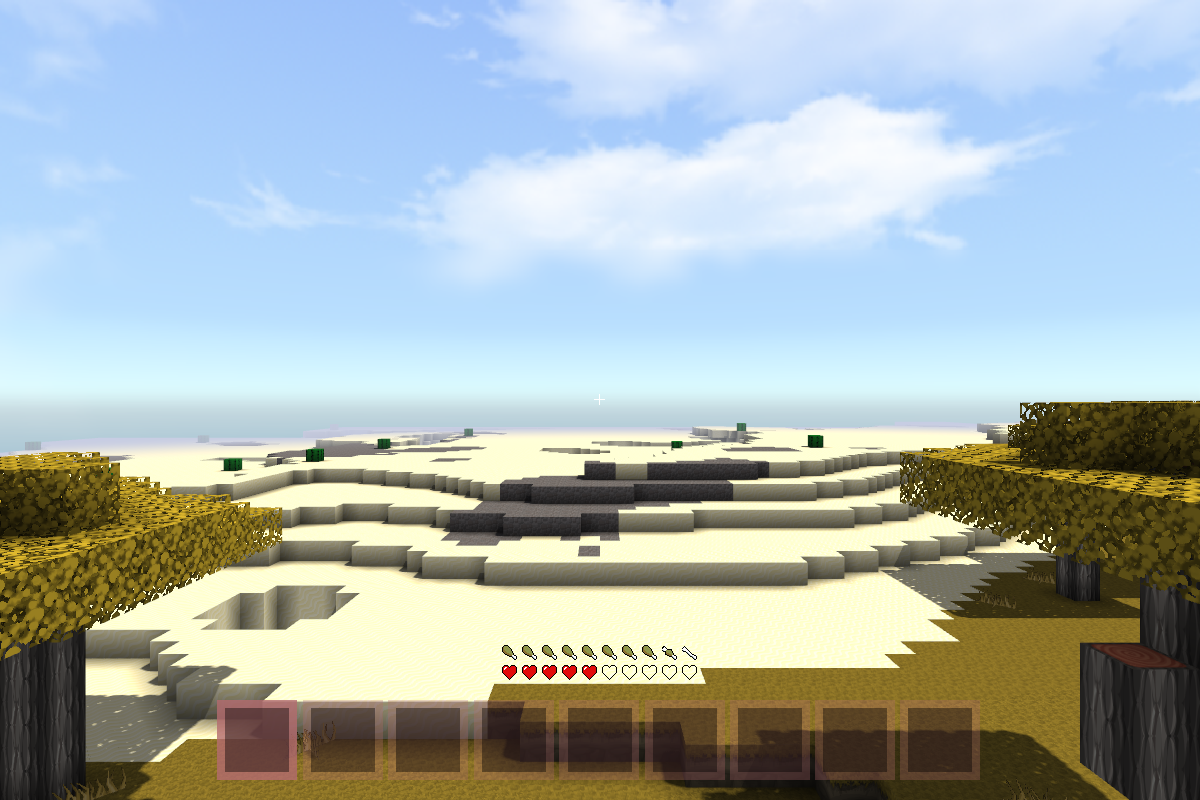
\includegraphics[width=.49\textwidth]{seed-2.png}
	\caption{Links: Seed 0. Rechts: Seed 2}\label{fig:static}
\end{figure}
Damit SystemA und SystemB bei Messungen mit Terrain-Generierung vergleichbar sind, wird in beiden Systemen der selbe Seed verwendet, wodurch die selbe Welt generiert wird. Abbildung~\ref{fig:static} zeigt zwei Screenshots von generierten Welten. Das linke Bild zeigt die mit dem Seed $0$ generierte Welt, das rechte Bild nutzt als Seed $2$. Hier sieht man beispielhaft, dass bereits kleine Unterschiede im Seed völlig andere Welten erzeugen. Für die folgenden Messungen wird der Seed $0$ verwendet. 

Im Szenario Welt-Statisch bleibt die Kamera wie in den vorherigen beiden Szenarien an ein und der selben Stelle.



\paragraph{\ac{fps}}
\begin{figure}[!htbp]
	\fpsplot{seed-0-static}
	\caption{Seed 0 Statisch}\label{fig:seed-0-static-fps}
\end{figure}
Der Verlauf der \ac{fps} in diesem Szenario ist in Abbildung~\ref{fig:seed-0-static-fps} abgebildet. Vergleicht man die Framerate mit denen der vorherigen Szenarien, lässt sich erkennen, dass die Startphase sich in beiden Systemen verlängert. SystemA benötigt \SI{20}{\second} statt \SI{15}{\second}, um eine konstante Framerate von etwa \SI{201}{\fps} zu erreichen. SystemB erreicht einen stabilen Zustand nach etwa \SI{22}{\second} mit durchschnittlich \SI{468}{\fps}.
Beide Systeme benötigen mit Terrain-Generierung also etwa \SI{5}{\second} länger für den Start. SystemB erreicht nach dem Start eine um \SI{133}{\percent} gesteigerte Framerate gegenüber SystemA. Dieser Wert liegt zwischen den gemessenen Werten der ersten beiden Szenarien.

\paragraph{\ac{cpu}}
Unter Betrachtung der \ac{cpu}-Auslastung im Welt-Statisch Szenario, die in Abbildung~\ref{fig:seed-0-static-cpu} zu sehen ist, lässt sich der zusätzliche Aufwand für die Terrain-Generierung der Welt ebenfalls erkennen.
\begin{figure}[!htbp]
	\cpuplot{seed-0-static}
	\caption{Seed 0 Statisch}\label{fig:seed-0-static-cpu}
\end{figure}
Während des Starts der Blocklib lasten beide System die \ac{cpu} bis zu \SI{97}{\percent} aus. Nach dem Start fällt die Auslastung in beiden Systemen, auf durchschnittlich \SI{13}{\percent} in SystemA und \SI{23}{\percent} in SystemB.
SystemB führt im Vergleich zu SystemA in diesem Szenario also zu einer um \SI{77}{\percent} erhöhten Auslastung der \ac{cpu}. SystemB lastet die \ac{cpu} in diesem Szenario mehr aus als in den Szenarien ohne generierter Welt. SystemA dagegen erreicht nach dem Start eine zu den bisherigen Szenarien vergleichbare Auslastung.

\paragraph{\ac{gpu}}
\begin{figure}[!htbp]
	\gpuplot{seed-0-static}
	\caption{Seed 0 Statisch}\label{fig:seed-0-static-gpu}
\end{figure}
Der zeitliche Verlauf der \ac{gpu}-Auslastung von Szenario 3 ist in Abbildung~\ref{fig:seed-0-static-gpu} zu sehen.

\paragraph{\ac{ram}}
\begin{figure}[!htbp]
	\memplot{seed-0-static-single-mem.csv}
	\memplot{seed-0-static-multi-mem.csv}
	\caption{Seed 0 Statisch}\label{fig:seed-0-static-mem}
\end{figure} 
